\documentclass[
	10pt,
	a4paper,
	% kosection,
	% footnote,
	% nobookmarks,
	% microtype,
	figtabcapt,
%	lwarp
]{oblivoir}

%%%%%%%%%%%%%%%%
% Front Matter %
%%%%%%%%%%%%%%%%

% \usepackage[usenames,dvipsnames]{color}

\usepackage[dvipsnames]{xcolor}

\usepackage{fapapersize}
\usefapapersize{*,*,30mm,*,35mm,*}
\definefageometry{default}{30mm,*,35mm,*}[\nopagecolor]
\definefageometry{test}{15mm,25mm,35mm,*}[\pagecolor{cyan!15}]


\usepackage{kotex-logo}

%for reference
\usepackage{hyperref}
\hypersetup{colorlinks=true, linkcolor=black, urlcolor=cyan}
\renewcommand{\figureautorefname}{그림~}
\renewcommand{\tableautorefname}{표~}
% \renewcommand{\sectionautorefname}{foobar}
% \renewcommand{\subsectionautorefname}{foobarbaz}

\usepackage{afterpage}
\usepackage{oblivoir-misc}
\usepackage{graphicx}
\usepackage{fancyvrb}

\usepackage{fontspec-xetex}
\usepackage{tabularx}

% \def\figureautorefname{그림~}

% for citaiton
% \usepackage{biblatex}
							% Declare packages

%%%%%%%%%%
% Title, Authors, Date %
%%%%%%%%%%

\title{패턴인식 보고서}
\author{120220210 고재현}
\date{\today}

\begin{document}

%%%%%%%%%%
% covers %
%%%%%%%%%%


%%%%%%%%%%%%%%%%%%%%%
% Table of Contents %
%%%%%%%%%%%%%%%%%%%%%
\maketitle

% \begin{abstract}
% 이 문서는 2022 인공지능개론(EEE4178) 과목의 설명서이다.

% \end{abstract}

\pagenumbering{roman}                           % Start page numbering in Roman numerals
% \tableofcontents*        						% Add table of contents
% \clearpage

%%%%%%%%%%%%%%%%%
% preliminaries %
%%%%%%%%%%%%%%%%%

\setcounter{table}{0}		                    % Reset table counter
\setcounter{figure}{0}		                    % Reset figure counter

%%%%%%%%%%%%%
% Main Text %
%%%%%%%%%%%%%

\pagenumbering{arabic}							% Start page numbering in Arabic numerals


\section{개요}{\label{sec:intro}}

\subsection{프로젝트의 목적}
\begin{itemize}\tightlist
    \item 다양한 폰트로 구성된 영문자 및 숫자를 분류하는 문제를 딥러닝을 이용하여 해결한다.
    \item 프로젝트를 통해 다음과 같은 내용을 학습한다.
    \begin{enumerate}[(1)]\tightlist
        \item 딥러닝을 이용한 문제해결을 위한 프로젝트 구조를 이해한다.
        \item 목적에 맞는 딥러닝 모델을 구성할 수 있다.
        \item 딥러닝 모델을 학습시킬 수 있다.
    \end{enumerate}

\end{itemize}



% \begin{figure}[htp]
%     \centering
%     \includegraphics[width=0.8\textwidth]{figures/data_ex.png}
%     \caption{데이터 예시}
%     \label{fig:data_ex}
% \end{figure}


\section{논문 요약}{\label{sec:review}}

\subsection{Multi-modal fusion transformer for end-to-end autonomous driving}{\label{subsec:Transfuser}}
\begin{figure}[htp]
    \centering
    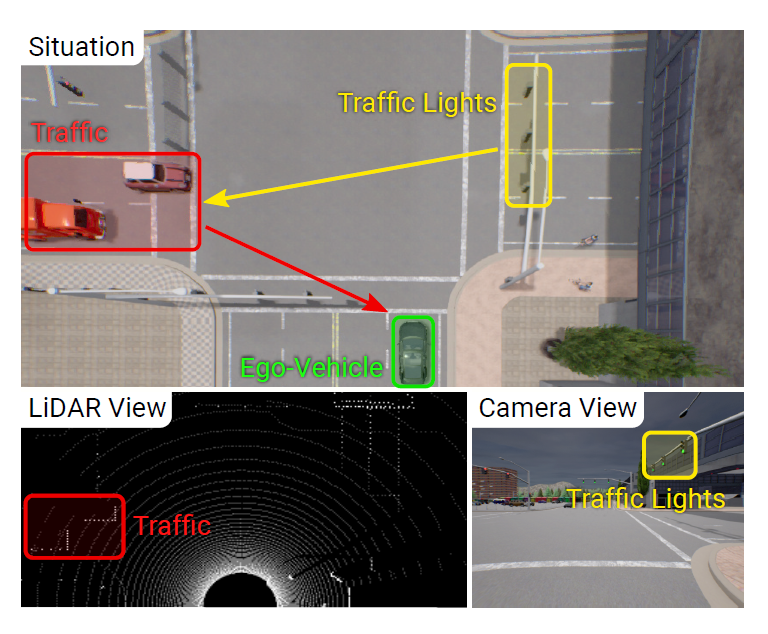
\includegraphics[width=0.5\textwidth]{figures/Transfuser_case.png}
    \caption{논문에서 해결하려는 문제 상황}
    \label{fig:tf_case}
\end{figure}
이 논문은 \autoref{fig:tf_case} 의 상황처럼
라이다(LiDAR : Light Detection And Ranging) 센서로 얻을 수 있는 주변의 차량의 위치에 따른 교통정보와
카메라로 얻을 수 있는 신호기에 따른 교통정보가 다른 경우,
두 센서로부터 얻을 수 있는 정보를 결합하여 차량의 주행을 제어하는 것을 목적으로 한다.
\begin{figure}[htp]
    \centering
    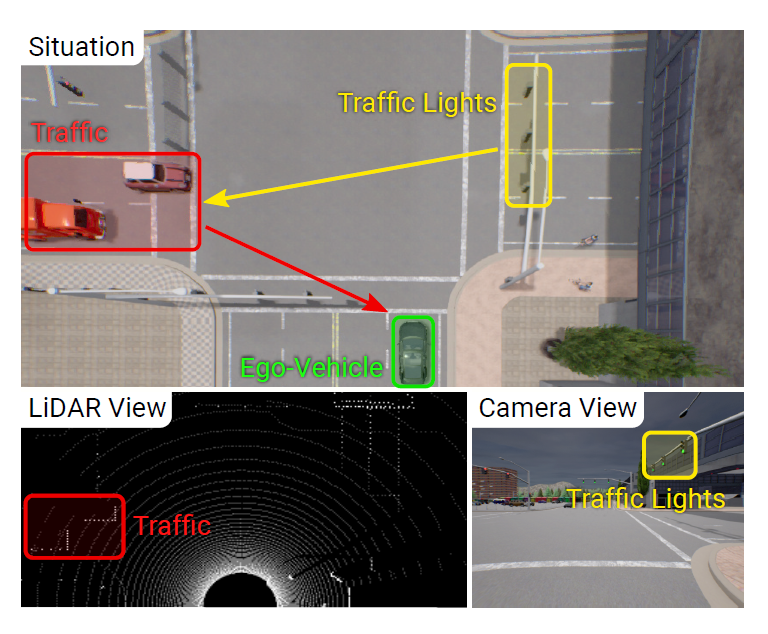
\includegraphics[width=\textwidth]{figures/Transfuser.png}
    \caption{Transfuser 구조}
    \label{fig:tf}
\end{figure}
\autoref{fig:tf}는 Transfuser의 구조를 보여준다.
두 센서의 출력으로부터 Resnet 구조\cite{Resnet}를 이용하여 정보를 추출하는 과정에서,
각 layer의 출력단으로부터 추출된 정보를 Transformer\cite{Transformer}를 이용하여 결합하는 것을 확인할 수 있다.

\subsubsection{Method}{\label{subsubsec:tf_method}}
% 목적, 입력, 전처리, 출력, 학습, 평가
\paragraph*{목적} 논문에서 제시한 목표는 시내 도로 주행에서의 point-to-point navigation이다.
point-to-point navigation은 차량이 목표지점까지
waypoint를 따라
교통법규를 지키면서
다른 차량과의 상호작용을 하며
완주하는 것을 의미한다.
이를 달성하기 위한 방법으로 강화학습 기법 중 하나인 Imitation Learning을 채용하였다.
Imitation Learning은 전문가가 직접 주행한 데이터를 따라하도록 agent의 policy를 학습하는 것을 의미한다.

\paragraph*{입출력} 자율주행 오픈소스 시뮬레이터 CARLA\cite{CARLA}에 있는 urban 가상환경에서 수집한 데이터를 입출력으로 사용하였다.
\textbf{입력}은 두 가지로, 카메라와 라이다 센서의 출력이다.
카메라로부터 얻은 영상의 왜곡을 줄이기 위해 이미지 입력의 중앙을 잘라내어 $256 \times 256 \times 3$  크기로 사용했다.
LiDAR 센서의 출력 또한 주변부분의 정보를 기반으로 $256 \times 256 \times 2$ 사이즈로 잘라내어 사용하였다.
채널의 한쪽은 지면 위, 한쪽은 지면 아래를 의미한다.
\textbf{출력}은 PID controller로 차량을 제어하기 위해 4개의 waypoint $\{w_t = (x_t, y_t)\}_{t=1}^T$ 로 설정했다.

\paragraph*{모델}
모델은 \autoref{fig:tf}에서 두 가지 부분으로 나눌 수 있다.
첫째는 Resnet과 Transformer를 이용하여 구성한 Multi-Modal Fusion Transformer(Transfuser)이고,
둘째는 MLP와 GRU로 구성된 Waypoint Prediction Network이다.
먼저 Transfuser의 동작을 살펴보자.
전반적인 동작은 \autoref{subsec:Transfuser} 의 표제 문단에서 작성하였으므로 Transformer의 적용 방법만을 확인한다.
Transformer로는 GPT 모델을 사용하였다.
\begin{enumerate}\tightlist
    \item 라이다 입력과 영상 입력에 대해 컨볼루션과 풀링을 진행하여 채널 수를 늘리면서 특징을 추출한다.
    \item 특징의 크기를 average pooling을 통해 8x8 로 줄인다.
    \item 각 특성맵을 concat하여 16x8 크기의 특성맵을 만든다.
    \item velocity를 value로, 16x8 특징을 key와 query로 사용하여 self attention(dot product attention)을 적용한다.
    \item bilinear interpolation을 통하여 원본 영상의 크기로 확대한다.
    \item 이전 단의 특성맵과 attention을 통해 추출한 특성맵을 더하여 특성맵을 업데이트한다.
\end{enumerate}
둘째로 Waypoint Prediction Network의 동작을 살펴보자.
\begin{enumerate}\tightlist
    \item activation이 ReLU인 3-Layer Perceptron을 이용하여
    $1 \times 1 \times 512$ 크기의 특징을
    $1 \times 1 \times 64$ 크기의 특징으로 압축한다.
    \item 압축된 특징을 GRU에 입력하여 4개의 waypoint를 예측한다.
\end{enumerate}
\paragraph*{학습}
모델의 Loss는 전문가의 주행 데이터와의 L2 distance를 사용하였다. 

\subsubsection{result}
\begin{figure}[htp]
    \centering
    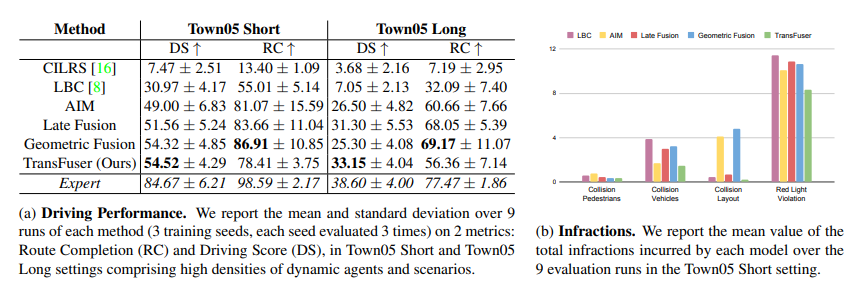
\includegraphics[width=\linewidth]{figures/Transfuser_result.png}
    \caption{Transfuser 실험 결과}
    \label{fig:tf_res}
\end{figure}
\autoref{fig:tf_res} 에서 Transfuser의 실험 결과를 확인할 수 있다.
왼쪽 장표는 주행 완료도와 안전운전 정도를 나타낸 것이고,
오른쪽 막대그래프는 사고율을 나타낸 것이다.
비교한 방법들에 비해 주행의 완료도도 좋아지고,
안전운전의 정도도 좋아졌고,
사고율도 줄어든 것을 확인할 수 있다.

\subsubsection{Discussion}
이 논문은 앞서 \autoref{sec:review} 의 첫 문단에서 밝힌 바와 같이
교통신호 인식과 차량 및 보행자 인식을 동시에 처리하는 방식을 제안하였다.
이는 수업에서 다룬 패턴인식 과정과는 달리 raw data로부터 feature를 구하는 과정마저
network에게 맡긴 것으로 볼 수 있지만, 다차원의 입력의 차원을 줄이고,
그로부터 원하는 결과물을 얻는다는 점에서 수업의 내용과 맥락을 같이한다.
수업의 6장에서 다룬 neural network의 대부분의 내용을 포함하고 있다.
\begin{itemize}\tightlist
    \item criterion function으로 2차 minkowski distance를 사용
    \item multi-layer perceptron을 사용하여 정보 압축
\end{itemize}


\subsection{YOLOv7: Trainable bag-of-freebies sets new state-of-the-art for real-time object detectors}{\label{subsec:yolov7}}

asdf
% \section{프로젝트 일정 및 제한 사항}{\label{sec:schedule}}

\subsection{제출 기한}
\begin{itemize}\tightlist
    \item 제출 마감 : 12월 18일 (일) 자정(23:59), 지각 제출에 대한 감점 있음
    \item 지각 제출 기한 : 12월 20일 (화) 자정 (23:59), 일당 5점씩 감점, 이후 제출 불가
\end{itemize}


\subsection{제한 사항}
    \begin{itemize}\tightlist
            \item 모델의 학습 관련
            \begin{itemize}\tightlist
                \item 모델은 Google Colab에서 제공하는 GPU 기준 \textcolor{red}{10분 이내에 학습 완료}되어야 한다.
                \item Train 시간이 10분 이상일 시 초과 시간에 따라 감점한다.
            \end{itemize}
        \item 모델 관련
            \begin{itemize}\tightlist
                \color{red}
                \item Pretrained model은 사용 불가능하다.
                \item 모델 구조는 분류 분야의 논문을 참고해서 구성해도 좋으나, torch 또는 torchvision 등을 통해 불러오지 않고 직접 구현해야 한다. 
                \item Torch에서 (대체로 Pretrained model과 함께) 제공하는 ResNet이나 MobileNet, Transformer 따위의 모델을 불러와서 사용하는 것은 불가능하다.
            \end{itemize}
        \item 라이브러리 관련
            \begin{itemize}\tightlist
                \item Python 표준 라이브러리, Pytorch, Numpy 제공 라이브러리만 모델 구성 및 학습에 사용 가능하다.
                \item Matplotlib, Seaborn 등 시각화를 위한 라이브러리는 자유롭게 활용해도 좋다.
                \item 언급된 것 외의 학습성능 향상을 위한 라이브러리 사용 시 조교에게 문의하여라.
            \end{itemize}
        \item 데이터 관련
            \begin{itemize}\tightlist
                \item 데이터 전처리는 자유롭게 진행할 수 있다.
                \item 데이터로더는 \href{https://github.com/jaehyun-ko/EEE4178-Project-2022/blob/main/src/Project_2022_utils.ipynb}{프로젝트 도구}에서 제공된 것을 가공하지 않고 사용한다.
            \end{itemize}
    \end{itemize}

% \section{제출 형태 및 채점 기준}{\label{sec:eval}}

\subsection{제출 형태}
아래의 파일들을 \textcolor{RubineRed}{PJ\_학번.zip} 으로 압축하여 제출한다. (예: PJ\_20181485.zip)
\\ \textcolor{Red}{파일명 및 확장자가 잘못될 경우 감점 있음}
\begin{enumerate}\tightlist
    \item Train에 사용된 주피터 노트북 : \textcolor{RubineRed}{train\_학번.ipynb}
    \begin{itemize}
        \item Train 시 할당받은 GPU의 종류를 확인할 수 있도록
        \href{https://github.com/jaehyun-ko/EEE4178-Project-2022/blob/main/src/Project_2022_utils.ipynb}{프로젝트 도구}에서 제시한 방법대로
        \textcolor{Orange}{!nvidia-smi} 셀 및 출력을 포함한다.
        \item Train의 수행 시간 또한 측정하여 출력한다.
    \end{itemize}
    
    \item Train 후 저장된 model : \textcolor{RubineRed}{학번.pth}
    \item Test에 사용할 파이썬 스크립트 : \textcolor{RubineRed}{test\_학번.py}
    \\train 을 통해 저장한 모델을 불러와서 동작하도록 작성하되, Test set이 주어져 있지 않으므로 Validation set을 test하도록 작성한다.
    \item 보고서 : \textcolor{RubineRed}{project\_학번.pdf}
        \begin{itemize}
            \item 보고서는 다음 내용을 포함한다.
            \begin{enumerate}[1.]
                \item 과제 목표
                \item 배경 이론
                \item 과제 수행 방법
                \item 결과 및 토의
                \\ 할당받은 GPU 종류 및 학습에 사용된 시간을 기재한다. 예를 들어 \textcolor{Orange}{Tesla T4 환경에서 2.003초}
                % 이거 flops 계산으로 변경 해 주세요!!
                \item 참고 문헌
            \end{enumerate}
        \end{itemize}
\end{enumerate}

\subsection{채점 기준}
    \begin{itemize}\tightlist
        \item Model Accuracy (순위) : 50\%
        \item 프로젝트 보고서 : 50\%
    \end{itemize}



% \input{text/appendix.tex}



%%%%%%%%%%%%%%%%%%%%%%
% References Section %
%%%%%%%%%%%%%%%%%%%%%%
\bibliographystyle{ieeetr}						% Declare bibliography style
\bibliography{ref.bib}							% Declare bibliography file

\clearpage

\end{document}
